\documentclass[a4paper,twoside]{memoir}
\usepackage[utf8]{inputenc}
\usepackage[british]{babel}
\usepackage{csquotes}
\usepackage[T1]{fontenc}
\usepackage{charter}
\usepackage[bitstream-charter]{mathdesign}
\usepackage[final,babel]{microtype}
\usepackage[hidelinks,pdfpagelayout=TwoPageRight]{hyperref}
\usepackage{xcolor}
\usepackage{menukeys}
\usepackage{minted}
\usepackage{amsmath}
\usepackage{enumitem}
\usepackage{siunitx}
\usepackage{booktabs}
\usepackage{makeidx}

\newcommand{\FrameTitle}[2]{%
  \fboxrule=\FrameRule \fboxsep=\FrameSep
  \fbox{\vbox{\nobreak \vskip -0.7\FrameSep
    \rlap{\centerline{\strut#1}}\nobreak\nointerlineskip% centered
    \vskip 0.7\FrameSep
    \hbox{#2}}}}
\newenvironment{framewithtitle}[2][\FrameFirst@Lab\ (cont.)]{%
  \def\FrameFirst@Lab{\textbf{#2}}%
  \def\FrameCont@Lab{\textbf{#1}}%
  \def\FrameCommand##1{%
    \FrameTitle{\FrameFirst@Lab}{##1}}%
  \def\FirstFrameCommand##1{%
    \FrameTitle{\FrameFirst@Lab}{##1}}%
  \def\MidFrameCommand##1{%
    \FrameTitle{\FrameCont@Lab}{##1}}%
  \def\LastFrameCommand##1{%
    \FrameTitle{\FrameCont@Lab}{##1}}%
\MakeFramed{\advance\hsize-\width \FrameRestore}}%
{\endMakeFramed}

\newcounter{exercisectr}
\newenvironment{exercise}
{\stepcounter{exercisectr}\begin{framewithtitle}{Practical \arabic{exercisectr}}}
{\end{framewithtitle}}

\newenvironment{py}{\begin{minted}{python}}{\end{minted}}

\newcommand{\shellcmd}{\texttt}
\newcommand{\shellvar}[1]{$\langle \text{#1}\rangle$}
\newcommand{\additional}{\medskip\noindent{\textit{Additional exercises}}}
\newcommand{\TODO}[1]{\textcolor{purple}{TODO: \emph{#1}}}
\newcommand{\home}{\raise.17ex\hbox{$\scriptstyle\mathtt{\sim}$}}

\setlist[itemize]{leftmargin=*,label={--}}

\makeindex

\begin{document}
\tableofcontents*

\chapter{The Linux command line}
\label{chap:linux}

\section{Linux commands}

\begin{itemize}
\item Linux offers a command line which allows you to manipulate files, process data, and perform almost any other operation
\item Some commands take options that modify their behaviour.  Options usually start with one hyphen (\shellcmd{-}) or two hyphens (\shellcmd{-{}-}), and appear after the command name.  Options are separated by spaces.
\item Some commands take one or more arguments which often specify the location of a file or directory.  Arguments come after the command and any options, and are also separated by spaces.
\item A typical command with options and arguments might look like this:
\begin{minted}{bash}
$ sort --numeric-sort -r dataSet2013.txt dataSet2014.txt
\end{minted}
\item Most commands come with manuals, called `man pages'; if you know the name of the command, \shellcmd{man \shellvar{mycommand}} displays its man page.  Type \keys{q} to return to the command line.
\index{man@\shellcmd{man}}
\item Most commands display their results on the command line.  If instead you want to save the output to a file, you can use output redirection (\shellcmd{>}).  For example
\index{Redirection}
\begin{minted}{bash}
$ sort --numeric-sort dataSet2013.txt > sorted2013.txt
\end{minted}
\item Use \keys{ctrl+c} to abort a command that is currently running
\item Use \keys{ctrl+d} on a blank line when you have finished entering all the input to a command
\end{itemize}

\section{The file system}
\begin{itemize}
\item Linux has a single file system that comprises a tree of directories that contain files
\item The slash symbol (\shellcmd{/}) identifies the root of the tree
\item A pathname identifies a file or directory, which is the path that is taken through the directory tree to reach it
\item The slash symbol is also used to separate the names of files and directories in a pathname
\item An absolute path specifies a location starting from the root of the tree.  Hence, absolute paths always begin with a slash (\shellcmd{/}).
\item The command line remembers your current location in the directory tree, and you can discover its path with the \shellcmd{pwd} command (short for `Print Working Directory')
\item If a path does not start with a \shellcmd{/} then it gives a location that is relative to the current location.  Hence, it is called a `relative path'.
\item Files that belong to the user are stored in a location called the `home' directory which has the path \shellcmd{/home/\shellvar{username}}.  This is analagous to `My Documents' on Microsoft Windows.
\item To save typing the full path, the home directory has a special name, \home\ (the tilde character).
\end{itemize}

\subsection{Directory manipulation}
\begin{itemize}
\item The \shellcmd{ls} command lists the contents of the current directory
\index{ls@\shellcmd{ls}}
\item The \shellcmd{cd} command, short for `Change Directory', changes the current directory to a new location
\index{cd@\shellcmd{cd}}
\item \shellcmd{cd /home/alice/photos/} moves to the \shellcmd{photos} subdirectory in alice's home directory
\item If our current directory is \shellcmd{/home/alice/photos/}, the command \shellcmd{cd 2009/kenya} changes our current directory to \shellcmd{/home/alice/photos/2009/kenya/}
\item To move up a level in the directory tree, we can use the special directory named with two periods (\shellcmd{..})
\item \shellcmd{cd ..} moves up one level to \shellcmd{/home/alice/photos/2009/}
\item And then \shellcmd{cd ../../} moves up another two levels back to alice's home directory, \shellcmd{/home/alice/}
\item Many other commands also accept a pathname.  For example, \shellcmd{ls \home/photos} lists the contents of alice's photos directory (notice that we have used the special \home\ symbol).
\item \shellcmd{mkdir -p \shellvar{pathname}} creates a new directory (and will create any directories that don't already exist in the directory tree)
\index{mkdir@\shellcmd{mkdir}}
\end{itemize}

\subsection{File manipulation}
\begin{itemize}
\item Copy a file with the command \shellcmd{cp \shellvar{source} \shellvar{destination}}
\index{cp@\shellcmd{cp}}
\item Copy a directory and all of its contents with \shellcmd{cp -r \shellvar{source} \shellvar{destination}} (where the option \shellcmd{-r} specifies recursive copying)
\item To rename a file or directory, use \shellcmd{mv \shellvar{source} \shellvar{destination}}
\index{mv@\shellcmd{mv}}
\item The same command can be used to move a file or directory to another location in the tree.  For example, \shellcmd{mv photos/2009/kenya photos/2010/} moves the \shellcmd{kenya} directory into the \shellcmd{2010} directory.
\item To delete a file, use \shellcmd{rm \shellvar{file}}
\index{rm@\shellcmd{rm}}
\item To delete a directory and all its contents, first decide if you really want to do this.  There is no Recycle Bin to rescue you.  If you really must, use \shellcmd{rm -r -I \shellvar{directory}}.
\end{itemize}

\begin{exercise}
\begin{enumerate}
	\item Launch a terminal as shown in figure~\ref{fig:term}.  Check that the current directory is your home directory using the \shellcmd{pwd} command.
	\item Create a new subdirectory.  In future practicals, we will store our Python code in this new directory.  You might want to give it a path such as \shellcmd{\home/mpecdt/python/practicals}, or whatever you prefer.
	\item Run the \shellcmd{gedit} text editor by using the Ubuntu launcher and save a text file to the new directory.
	\item Try copying, renaming, and moving the new file to anywhere in your home directory.  As you do this, you might want to \shellcmd{cd} to different directories.  Alternatively, you can stay in the same directory and pass relative paths as arguments to the commands.
	\item Remembering that there is no Recycle Bin on the linux command line, remove the file using the \shellcmd{rm} command.
\end{enumerate}
\end{exercise}

\begin{figure}
	\centering
	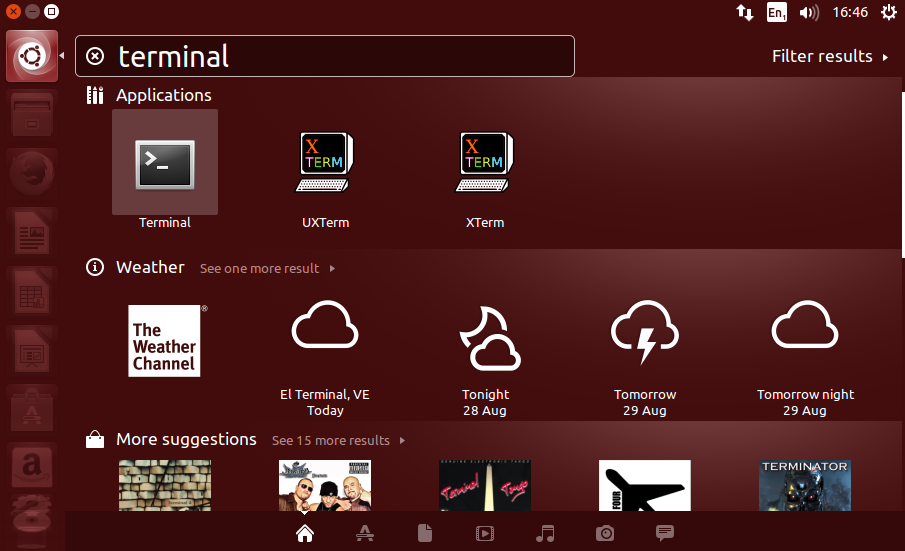
\includegraphics[width=\textwidth]{terminal.png}
	\caption{Launching a terminal in Ubuntu}
	\label{fig:term}
\end{figure}

\begin{exercise}
Try sorting a list of numbers.  The \shellcmd{sort} command takes its input from the command line and expects each list item on a new line.  Try entering the following
\index{sort@\shellcmd{sort}}
\begin{minted}{bash}
$ sort --numeric-sort
11.4
11.2
-2
4
\end{minted}
Type \keys{\ctrl+d} on an empty line when you have finished entering the list.  The result should be printed to the command line.

If you make a mistake entering the data, you can abort the \shellcmd{sort} command by typing \keys{\ctrl+c}.  Notice that no sorting is performed and nothing is printed to the command line.

\additional

In the previous exercise we used the \shellcmd{-{}-numeric-sort} option to sort items numerically.  The \shellcmd{sort} command has many other options that control the way data is sorted.

Try sorting words in reverse alphabetical order, ignoring upper and lower cases.  To find the appropriate options, take a look at the manual page with \shellcmd{man sort}, and type \keys{q} to get back to the command line prompt.

The output of one command can be used as the input to another using a pipe (\shellcmd{|}).  To remove duplicate items in a list, we can sort them, then remove adjacent lines that are the same.  Try the following command
\begin{minted}{bash}
$ sort | uniq
bob
alice
charlie
bob
charlie
\end{minted}
using \keys{ctrl+d} when you have finished entering the list.
\end{exercise}

\chapter{The Python programming language}

\section{Installing Python on Ubuntu 14.04}
\label{sec:installation}

\begin{enumerate}
\item Launch the terminal application as shown in Figure~\ref{fig:term}.  You should see a command line with a flashing prompt.
\item Enter the command \shellcmd{sudo apt-get install ipython3 python3-tk python3-pytest python3-scipy}.  You will be prompted to enter your password.  Enter \keys{Y} when prompted to continue.
\item To test that Python is working, run the \shellcmd{ipython3} command.  Your terminal window should look something like Figure~\ref{fig:ipython3}.  Try evaluating an expression at the IPython prompt, such as \shellcmd{3 + 5}.  You can return to the linux command line by typing \keys{\ctrl+d}.
\item Launch a text editor by searching for `gedit' in the Ubuntu launcher.  Choose \menu{Edit > Preferences > Editor}.  Enable \menu{Insert spaces instead of tabs} and set \menu{Tab width} to 4.  The configuration is shown in figure~\ref{fig:gedit}.
\end{enumerate}

\begin{figure}
	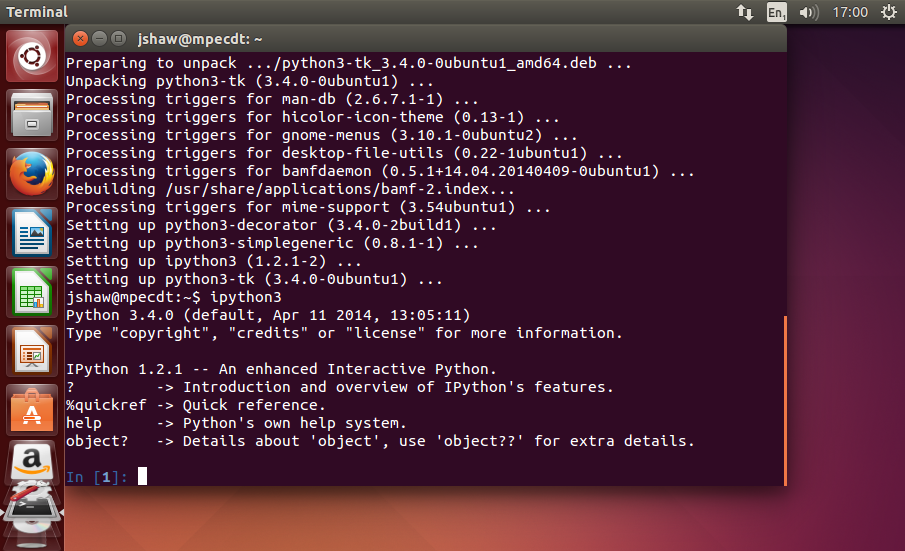
\includegraphics[width=\textwidth]{ipython3.png}
	\caption{The \shellcmd{ipython3} prompt}
	\label{fig:ipython3}
\end{figure}

\begin{figure}
	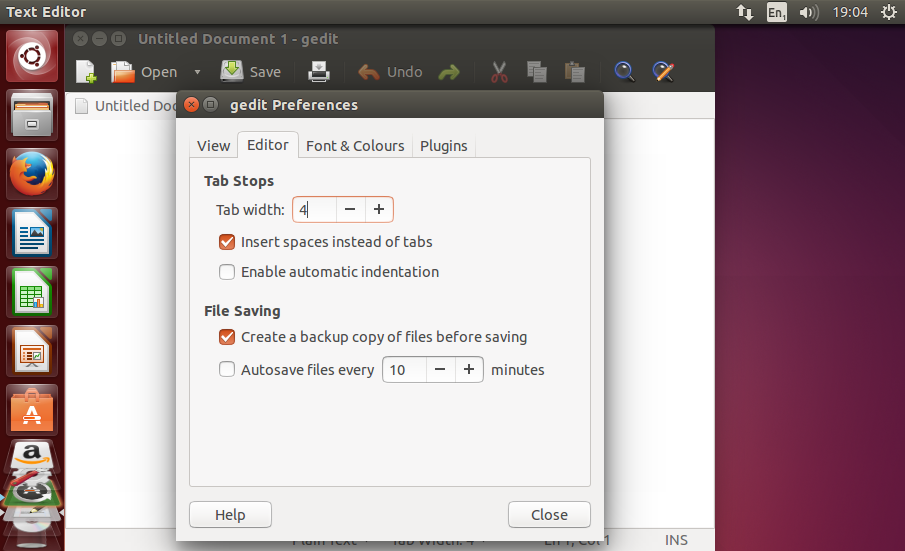
\includegraphics[width=\textwidth]{gedit.png}
	\caption{Configuring the \shellcmd{gedit} text editor}
	\label{fig:gedit}
\end{figure}


\section{Numeric data}
\begin{itemize}
\item There are many different types of data in Python including numeric, textual, and boolean (true or false) data types
\item There are three numeric types built into Python
	\begin{description}
	\item[Integer values ($\mathbb{Z}$)]{Examples of integer values are \shellcmd{5} and \shellcmd{-8}.  Unlike some other programming languages, integers in Python have no minimum or maximum value.}
	\item[Real values ($\mathbb{R}$)]{In Python these are called `floating point' numbers, or just `floats'.  Examples of floats are \shellcmd{5.9}, \shellcmd{13.0} and \shellcmd{-2.39e-12} (where \shellcmd{e} means `exponent', so $\text{\shellcmd{-2.39e-12}} = \num{-2.39e-12}$).  Because floats have limited precision, they can only approximate real numbers, and rounding errors often appear when we do arithmetic with floating point values.  We will explore these pitfalls in Practical~\TODO{xref}.}
	\item[Complex values ($\mathbb{C}$)]{Not covered in this course, but details can be found at \url{https://docs.python.org/3/library/stdtypes.html#typesnumeric}}
	\end{description}
\item Python provides a variety of numeric operators including addition (\shellcmd{+}), subtraction (\shellcmd{-}), multiplication (\shellcmd{*}), division (\shellcmd{/}) and exponentiation (\shellcmd{**})
\item Values can be combined with operators to form expressions.  Python can evaluate expressions and print the result to the command line.  For example, \shellcmd{3 + 6 * -2} prints \shellcmd{-9}, and \shellcmd{5.3 ** 2.5} prints \shellcmd{64.66803638583747}.
\item Python uses the conventional order of operations such that multiplication has a higher precedence than addition, for example.  To make the expression clearer, or to force a different order of evaluation, you can use parentheses.  For example, \shellcmd{(3 + 6) * -2} prints \shellcmd{-18}.  For full details of operator precedence, see \url{https://docs.python.org/3/reference/expressions.html#evaluation-order}.
\end{itemize}

\begin{exercise}
For this practical, you will need to use the IPython interactive shell.  Execute it at the command line using \shellcmd{ipython3}.  If you want to recall lines you typed previously, you can use the \keys{\arrowkeyup} and \keys{\arrowkeydown} arrow keys.
\begin{enumerate}
\item Try evaluating \shellcmd{12345678901234567890 + 1234567890123456789}.  Now try evaluating \shellcmd{12345678901234567890.0 + 12345678901234567890.0}.  Can you explain why the answers differ?  What is the significance of the decimal place?

\item Try evaluating $3 \div 10$.  Do you get the expected answer?  Now try evaluating $1 \div 10 \times 3$.  Can you explain why the answer is different?

\item Try evaluating \shellcmd{10 + 1e17}.  Why is the answer incorrect?  Can you write a different expression that gives the correct result? % 10 + (10 ** 17)
\end{enumerate}
\end{exercise}

\section{Boolean logic}
\begin{itemize}
\item Another of Python's data types is the boolean type.  Its two values are \shellcmd{True} and \shellcmd{False}.
\index{false@\shellcmd{False}}
\index{true@\shellcmd{True}}
\item We can evaluate boolean expressions using the boolean operators \shellcmd{and}, \shellcmd{or} and \shellcmd{not}.  For example, \shellcmd{not True} evaluates to \shellcmd{False}.  \shellcmd{True or False} evaluates to \shellcmd{True}.
\index{and@\shellcmd{and}}
\index{or@\shellcmd{or}}
\index{not@\shellcmd{not}}
\item Numeric expressions can be compared for equality or inequality using one of the following operators

\begin{tabular}{ c @{\hspace{2em}} c}
	\toprule
	Mathematical expression & Python expression \\ \midrule
	$3 = 4$			& \shellcmd{3 == 4} \\
	$3 < 4$			& \shellcmd{3 < 4} \\
	$3 \leq 4$		& \shellcmd{3 <= 4} \\
	$3 > 4$			& \shellcmd{3 > 4} \\
	$3 \geq 4$		& \shellcmd{3 >= 4} \\
	$3 \neq 4$		& \shellcmd{3 != 4} \\
	\bottomrule
\end{tabular}

All of these expressions will evaluate to a boolean value of either \shellcmd{True} or \shellcmd{False}.

\item We can construct more elaborate expressions.  For example, $3 < 4 \leq 5$ could be written in Python as \shellcmd{3 < 4 and 4 <= 5} or, more consisely, \shellcmd{3 < 4 <= 5}.

\item Because floats are only approximations, it is dangerous to test that they are equal (\shellcmd{==}) or not equal (\shellcmd{!=}).  When working with floating point numbers, you should almost always compare them for inequality (\shellcmd{<}, \shellcmd{<=}, \shellcmd{>}, \shellcmd{>=}).  
\end{itemize}

\section{Modules}
\begin{itemize}
\item The features we have covered so far are all built into the Python language itself.  Additional functions are provided by Python modules.  The standard Python implementation includes modules for common tasks including mathematical calculations, and reading and writing files.  Additional modules can be installed for more specialised tasks such as matrix solving and graph plotting.
\item To gain access to a module's functions, you must `import' them.  There are a few different ways to do this
\index{import@\shellcmd{import}}
\begin{enumerate}
	\item It is often useful to see what module a function belongs to.  We can make this evident by using a fully-qualified import.  For example
\begin{minted}{python}
import sys

print(sys.stdin.readline())
\end{minted}
	\item If the module name is longer, we might prefer to use a shorter name in our code:
\begin{minted}{python}
import numpy as np

print(np.dot(3, 4))
\end{minted}
	\item If it makes the code clearer, you might want to omit the module name from function calls:
\begin{minted}{python}
from math import ceil

print(ceil(3.5))
\end{minted}
	\item Furthermore, if we are using many functions from the same module, it is sometimes more convenient to write
\begin{minted}{python}
from math import *

print(floor(3.5))
\end{minted}
\end{enumerate}
\end{itemize}

\section{Mathematical functions}
\begin{itemize}
\item The \shellcmd{math} module provides a variety of common mathematical functions.  To gain access to these functions, you must `import' them from the module using the Python command
\index{math module@\shellcmd{math} module}
\begin{minted}{python}
from math import *
\end{minted}
\item The \shellcmd{math} module is documented at \url{https://docs.python.org/3/library/math.html}.  Some of the most common functions are summarised below

\index{floor@\shellcmd{floor()}}
\index{ceil@\shellcmd{ceil()}}
\index{exp@\shellcmd{exp()}}
\index{log@\shellcmd{log()}}
\index{log10@\shellcmd{log10()}}
\index{sqrt@\shellcmd{sqrt()}}
\index{abs@\shellcmd{abs()}}
\begin{tabular}{ c @{\hspace{2em}} c}
	\toprule
	Mathematical function	& Python function \\ \midrule
	$\lfloor 3.3 \rfloor$	& \shellcmd{floor(3.3)} \\
	$\lceil 3.3 \rceil$	& \shellcmd{ceil(3.3)} \\
	$e^{3.3}$		& \shellcmd{exp(3.3)} \\
	$\ln(3.3)$		& \shellcmd{log(3.3)} \\
	$\log(3.3)$		& \shellcmd{log10(3.3)} \\
	$\sqrt{3.3}$		& \shellcmd{sqrt(3.3)} \\
	$| -3.3 |$		& \shellcmd{abs(-3.3)}\footnotemark \\
	\bottomrule
\end{tabular}
\footnotetext{\shellcmd{abs()} is actually built into Python, and you do not need to import the \shellcmd{math} module to use it.}

\item The \shellcmd{math} module also includes trigonometric and hyperbolic functions, and also defines the constants $e$ and $\pi$.  For example, we could use them in expressions such as \shellcmd{e ** (-1/3)} or \shellcmd{sin(pi/2)}.
\end{itemize}

\section{Variables}
\begin{itemize}
	\item So far, our expressions have only contained fixed values (known as `literals' in Python)
	\item We can also store variable data.  A variable should be given a name that describes its purpose, such as \shellcmd{bank\_balance}, \shellcmd{user\_name} or \shellcmd{overdrawn}.  \textit{Can you suggest suitable data types for each of these variables?}
	\item Before we can use variables in an expression, we must assign a value.  Here are some examples of assignment statements:
\begin{minted}{python}
	bank_balance = -193
	user_name = "Joe Bloggs"
\end{minted}
	\item A variable's value can also be assigned by evaluating an expression.  For example, we can set the \shellcmd{overdrawn} variable like this:
\begin{minted}{python}
	overdrawn = bank_balance < 0
\end{minted}
	\item You can assign values to multiple variables.  If we wanted to define a point with coordinates $x, y, z$ we could write
\begin{minted}{python}
	(x, y, z) = 13.4, -2.8, 4.0
\end{minted}
	\item A variable can be given a new value using another assignment statement.  Although Python does not enforce it, it is good practice to assign values of the same data type.
	\item We can increment the value of a numeric variable like this
\begin{minted}{python}
	x += 5
\end{minted}
Which is equivalent to writing
\begin{minted}{python}
	x = x + 5
\end{minted}
Similarly, we can decrement, multiply, divide or exponentiate by placing the operator before the equals sign:
\begin{minted}{python}
	x -= 5
	x *= 3
	x /= 4.2
	x **= -1/2
\end{minted}
\end{itemize}

\section{Textual data}
\label{sec:textual}
\begin{itemize}
\item Python has a data type for textual data.  This type is called a `string' because it comprises a string of characters.
\item A string is enclosed in single or double quotes.  Examples of string values are \shellcmd{'hello world'} and \shellcmd{"The quick brown fox"}.
\item You can include placeholders in a string and use the \shellcmd{format} function to replace them with actual values.  For example
\index{format@\shellcmd{format()}}
\begin{minted}{python}
"The area of a circle with radius {r} is {area}" \
  .format(r=3, area=pi*3**2)
\end{minted}

Which will print
\begin{verbatim}
The area of a circle with radius 3 is 28.274333882308138
\end{verbatim}
Notice that, because the line was quite long, we have used a backslash so that we can continue the code on a second line.

\item If we want to control how values are formatted when they are printed as text, we can use a `format specifier'.  For example, if we want to display the area with 4 significant digits, we can use the format specifier \shellcmd{.4g} and write
\index{Format specifier}
\begin{minted}{python}
"The area of a circle with radius {r} is {area:.4g}" \
  .format(r=3, area=pi*3**2)
\end{minted}

Which will print
\begin{verbatim}The area of a circle with radius 3 is 28.27\end{verbatim}

\item There are many more ways to format data, for more information see \url{https://docs.python.org/3/library/string.html#formatspec}.

\item If you have a particularly long string, there are a couple of ways of writing them whilst keeping your code looking tidy
\begin{enumerate}
\item Use a multi-line string.  This is useful when you want to preserve line breaks in the text.  Multi-line strings are enclosed in three double quotes, for example
\begin{minted}{python}
"""An old silent pond...
A frog jumps into the pond,
splash! Silence again."""
\end{minted}
\item Alternatively, use can use the string concatenation operator (\shellcmd{+}).  This lets you split a long string onto several lines of source code:
\begin{minted}{python}
"An old silent pond... " + \
"A frog jumps into the pond, " + \
"splash! Silence again."
\end{minted}
This string will be printed on a single, long line.
\end{enumerate}

\item Sometimes you need to convert a string into a numeric type so that it can be used in calculations.  To create an integer, use \shellcmd{int()}.  To create a float, use \shellcmd{float()}.  For example:
\index{int@\shellcmd{int()}}
\index{float@\shellcmd{float()}}
\begin{minted}{python}
	int("-943") + 2
	float("3.5e7") * 100.0
\end{minted}
For more information, see \url{https://docs.python.org/3/library/functions.html#int} and \url{https://docs.python.org/3/library/functions.html#float}.
\end{itemize}

\begin{exercise}
Write some Python code that takes the mean of two real numbers.  The ceiling of the result should be displayed with two significant digits.  You might like to verify your code with these expected values:

\begin{tabular}{S S S}
	\toprule
	$a$ & $b$ & {Expected result} \\ \midrule
	5 & 12 & 9 \\
	250 & 20 & 1.4e2 \\
	-10.5 & 10.6 & 1 \\
	\bottomrule
\end{tabular}

\end{exercise}

\section{Source files}
\begin{itemize}
\item So far, we have only evaluated Python expressions using the interactive IPython shell.  However, complete programs are stored in files.  These are called `source files' since they contain the program's `source code'.  Python source file names have the suffix \shellcmd{.py}.
\item In linux, we must do two things to allow us to execute a Python source file:
\begin{enumerate}
	\item At the top of the file, add the line
\begin{minted}{bash}
#!/usr/bin/env python3
\end{minted}
	\item At the command line, we must issue the command \shellcmd{chmod +x \shellvar{source.py}} (\shellcmd{chmod} is short for `change mode', and \shellcmd{+x} means `enable execution')
\index{chmod@\shellcmd{chmod}}
\end{enumerate}
\item When we used the interactive console to evaluate expressions, the results were printed immediately.  However, we must use the \shellcmd{print()} function in a Python program.  For example, to print the area of a circle, as we did in section~\ref{sec:textual}, we could write the following program
\index{print@\shellcmd{print()}}
\begin{minted}{python}
#!/usr/bin/env python3
from math import *

print("The area of a circle with radius {r} is {area:.4g}" \
	.format(r=3, area=pi*3**2))
\end{minted}
\item If we save this source file to \shellcmd{\home/mpecdt-python/circle-area.py}, and \shellcmd{cd} to the \shellcmd{\home/mpecdt-python/} directory, we can execute our program on the command line like this
\begin{minted}{bash}
	$ ./circle-area.py
\end{minted}
\item Sometimes it is useful for a Python program to accept command line arguments (as described in chapter~\ref{chap:linux}).  For example, we might want to specify the radius on the command line.  The \shellcmd{sys} module lets us achieve this
\begin{minted}{python}
#!/usr/bin/env python3
from math import *
import sys

radius = float(sys.argv[1])

print("The area of a circle with radius {r} is {area:.4g}" \
	.format(r=radius, area=pi*radius**2))
\end{minted}
Now we can execute the program like this:
\begin{minted}{bash}
$ ./circle-area.py 4.5
The area of a circle with radius 4.5 is 63.62
\end{minted}
The \shellcmd{argv} variable is an array of strings.  We will describe arrays later in section~\ref{sec:arrays}.

\item If you have a lot of input data, it isn't convenient to provide it as a command line argument.  Instead, we can store the data in a file and use linux to send this data to our Python program.

We will modify our \shellcmd{circle-area.py} program to demonstrate this:
\index{readline@\shellcmd{readline()}}
\begin{minted}{python}
#!/usr/bin/env python3
from math import *
import sys

radius = float(sys.stdin.readline())

print("The area of a circle with radius {r} is {area:.4g}" \
	.format(r=radius, area=pi*radius**2))
\end{minted}
Now, to execute the program, we must create a text file containing the radius value, let's call it \shellcmd{radius.txt}.  Then we use the input redirection operator (\shellcmd{<}) like so
\index{Redirection}
\begin{minted}{bash}
$ ./circle-area.py < radius.txt
The area of a circle with radius 4.5 is 63.62
\end{minted}
\item If we wanted the result to be saved to a file, we could use output redirection operator (\shellcmd{>}) as well:
\begin{minted}{bash}
$ ./circle-area.py < radius.txt > area.txt
\end{minted}
\end{itemize}

\begin{exercise}
Using the code you wrote in Practical \TODO{xref}, create a complete Python program that has the same behaviour as before.  You should supply the two numbers as command line arguments.

\additional

Modify the program to read the two numbers from \shellcmd{stdin}.  Create a file with the two input numbers on separate lines and redirect Python to takes its input from this file.

Create two new files, each containing a single input number.  Using the \shellcmd{cat} command and a pipe (described in Practical~\TODO{xref}), use these files as input to your Python program.
\index{cat@\shellcmd{cat}}

Use the \shellcmd{tee} command to write the output to the command line and to a file.
\index{tee@\shellcmd{tee}}
\end{exercise}

\section{Indentation}
\index{Indentation}
\begin{itemize}
\item Unlike most languages, indentation is significant in Python.  Multiple lines of code are often grouped into `blocks' of code.  All code in a given block must have the same level of indentation.
\item In subsequent sections, we will discuss some of Python's control structures.  These include the loop structure, in which a block of code is executed zero or more times, and the \shellcmd{if ... else} structure, in which a code block is executed conditionally.
\item Usually, when you press \keys{\tab}, a special tab character is inserted into the source file.  When writing Python code, you must configure your text editor to insert spaces rather than tab characters.  If you are using \shellcmd{gedit}, we showed how to configure this text editor in section~\ref{sec:installation}.
\end{itemize}

\section{Functions}

\begin{itemize}
	\item We have already come across some functions provided by Python, such as \shellcmd{sqrt()} and \shellcmd{print()}.  We can also define our own functions in our Python programs.
	\item Functions in Python are somewhat more general that functions in mathematics because they do not need to take any input or return any output.
	\item The behaviour of a function has to be defined before it can be used in an expression.  We do this with the \shellcmd{def} keyword.  The behaviour of the function follows on subsequent indented lines.
\index{def@\shellcmd{def}}
	\item The most trivial function is one which has no input or output, and does nothing:
\begin{minted}{python}
def do_nothing():
	pass
\end{minted}
This function has the name \shellcmd{do\_nothing}.  It has just one line of code that defines its behaviour: we use the special \shellcmd{pass} keyword to instruct Python to do nothing.  We can call this function by writing \shellcmd{do\_nothing()}.
\index{pass@\shellcmd{pass}}
	\item A more interesting function takes one or more arguments.  For example, we can rewrite our circle area calculator as a function with two arguments:
\begin{minted}{python}
def print_circle_area(radius, area):
	print("The area of a circle " + \
	"with radius {r} is {area:.4g}" \
	.format(r=radius, area=area))

radius = 4.5
print_circle_area(radius, pi*radius**2)
\end{minted}
\item It is good practice to document functions using multi-line strings:
\begin{minted}{python}
def print_circle_area(radius, area):
	"""Print the specified radius and area of a circle.
	Radius is printed with Python default formatting.
	Area is formatted to four significant digits"""

	print("The area of a circle " + \
	"with radius {r} is {area:.4g}" \
	.format(r=radius, area=area))
\end{minted}

\item A function can also return a value.  Coming back to the circle area calculator, we can now rewrite the program as follows
\index{return@\shellcmd{return}}
\begin{minted}{python}
#!/usr/bin/env python3
from math import *

def circle_area(radius):
	return pi*radius**2

def print_circle_area(radius, area):
	print("The area of a circle " + \
	"with radius {r} is {area:.4g}" \
	.format(r=radius, area=area))

radius = 4.5
area = circle_area(radius)
print_circle_area(radius, area)
\end{minted}
\textit{Can you see a potential problem with the \texttt{print\_circle\_area()} function?  How might you improve it?}
\item Finally, you can create a function with a mixture of mandatory and optional arguments.  If an optional argument is omitted from a function call, a default value is used.  For example
\begin{minted}{python}
def wind_stress(u, rho_air=1.3, drag_coeff=10e-3):
	return drag_coeff * rho_air * u**2

print(wind_stress(10.0, 1.28, 8e-3))
print(wind_stress(10.0))
print(wind_stress(10.0, drag_coeff=8e-3))
\end{minted}
\label{wind-stress}
In the last example, notice how we specify the name of the \shellcmd{drag\_coeff} argument explicitly.  \textit{Can you see why this is necessary in this case?}
\end{itemize}

\section{Control structures}
\begin{itemize}
	\item We can evaluate boolean expressions to control which lines of code are executed.  For example
\index{if@\shellcmd{if}}
\index{else@\shellcmd{else}}
\begin{minted}{python}
bank_balance = -13

if bank_balance >= 0:
	print('In the black')
else:
	print('Overdrawn')
\end{minted}
Once again, we use indentation to specify the lines of code that belong to each case.
	\item If we need to test for more than one condition, we can use the \shellcmd{elif} keyword (a contraction of `else if')
\index{elif@\shellcmd{elif}}
\begin{minted}{python}
velocity = 23

if velocity < 0:
	print('Reverse gear')
elif velocity > 40:
	print('High gear')
elif velocity > 0:
	print('Low gear')
else:
	print('Neutral')
\end{minted}
Notice that we can use as multiple \shellcmd{elif} statements.
	\item If we need to execute the same code many times, we can use a control structure called a `loop'.  Python offers two loop types: the \shellcmd{while} loop and the \shellcmd{for} loop.  We discuss \shellcmd{for} loops later in section \TODO{xref}.
\index{loop}
	\item A \shellcmd{while} loop is used to repeatedly execute code until a given boolean expression evaluates to \shellcmd{True}:
\index{while@\shellcmd{while}}
\begin{minted}{python}
counter = 5
while counter > 0:
	print(counter)
	counter -= 1

print('Blast off!')
\end{minted}
\label{blast-off}
We will rewrite this more succinctly using a \shellcmd{for} loop in Practical \TODO{xref}.
\end{itemize}

\section{Python arrays}
\label{sec:arrays}
An array is a data structure that holds an ordered list of values.  We will look at two array implementations: first, Python's built-in array data type and, second, the array type provided by the \shellcmd{numpy} module.  In this section, we will look at Python's built-in arrays.

\subsection{Creation}
\begin{itemize}
\item We can create an array by surrounding a comma-separated list with square brackets.  Example arrays are \shellcmd{[5.8, 2.0, -4.3e2]}, \shellcmd{["bob", "charlie", "alice"]}, and \shellcmd{[]} (an array with no elements)

\item It is good practice to use the same data type for all array elements (for example, an array of integers, or an array of booleans, but not an array containing a mixture of integer and boolean elements)

\item You can `nest' arrays to create multi-dimensional array structures:
\begin{minted}{python}
my_square_matrix = [[1, 1, 1], [0, 2, 5], [2, 5, -1]]
\end{minted}

\item \index{range@\shellcmd{range()}} To create an integer sequence, use the \shellcmd{range()} function.  This function lets you specify the end of the sequence, the start and end, and an optional step.  Here are some examples:
\begin{minted}{python}
	range(3)         # [0, 1, 2]
	range(2, 5)      # [2, 3, 4]
	range(3, -7, -3) # [__________________________]
\end{minted} 
                         % [3, 0, -3, -6]
For more information on ranges, refer to \url{https://docs.python.org/3/library/stdtypes.html#range}
\end{itemize}

\subsection{Manipulation}
\begin{itemize}
\item To determine the number of elements in an array, use the \shellcmd{len()} function.  For example, \shellcmd{len([6, 2, 8])} evaluates to 3, and \shellcmd{len([])} evaluates to 0.
\item Array elements are indexed by number, starting at zero.  To get the value at a given index, we use square brackets again:
\begin{minted}{python}
a = [3, 0, -3, -6]
print(a[2])
\end{minted}
will print \shellcmd{-3}.

\item We can use the same indexing technique to assign a new value to a specific element
\begin{minted}{python}
a = [3, 0, -3, -6]
a[2] *= 4
print(a[2])
\end{minted}
will print \shellcmd{-12}.

\item Python provides a powerful tool, called `array slicing', that lets us access specific parts of an array.  There are several ways to slice an array\footnote{Source: \url{http://stackoverflow.com/a/509295/150884}}:
\index{Array slicing}
\begin{minted}{python}
my_array[a:b] # elements a (inclusive) to b (exclusive)
my_array[a:]  # all elements from a (inclusive) to array end
my_array[:b]  # all elements from array start to b (exclusive)
my_array[a:b:step] # elements a (inclusive) to b (exclusive) at each step
\end{minted}
where \shellcmd{a} and \shellcmd{b} are indexes into the array.
\item We can also use negative indexes with array slicing to index from the end of the array:
\begin{minted}{python}
my_array[-1]    # last element
my_array[-2:]   # last two elements
my_array[:-2]   # all except the last two elements
\end{minted}
\textit{How could you reverse a string using array slicing?}

\item Possibly the most common operation on arrays is `iteration', in which the same code is executed for each element in an array.  We can iterate over an array using a \shellcmd{for} loop.  To print the first few multiples of ten, we could write
\index{Iteration}
\index{range@\shellcmd{range()}}
\begin{minted}{python}
for i in range(5):
	print(10**i)
\end{minted}
\end{itemize}

% nesting?

\begin{exercise}
\begin{enumerate}
\item Turn the `Blast off!' example on page~\pageref{blast-off} into an executable source file

\item Modify the program to use a \shellcmd{for} loop

\item Put the countdown code into its own function which takes an argument for the starting number.

\item Make the starting number an optional argument that defaults to 5.

\item \index{Bisection method} The bisection method can be used to find the approximate solution to a function $f(x)$ such that the the error is less than the tolerance value $\epsilon$ (that is, $| f(x) | < \epsilon$).  Start with two values $a$ and $b$ such that $f(a) \leq f(x) \leq f(b)$.  At each iteration, find the midpoint $c = \left(a + b\right) / 2$ and calculate $f(c)$.  The function should terminate if $| f(c) | < \epsilon$ or the maximum number of iterations is reached.

Implement a root finding function using the bisection method.  Use it to find an approximate solution to $x^5 + x + 1 = 0$ using $a = -1.0$, $b = 1.0$, $\epsilon = \num{1e-6}$ and a suitable maximum number of iterations.  Name the function \shellcmd{find\_root(a, b, epsilon)} and save it in a source file named \shellcmd{find\_root.py}.

You might ask how to handle the case where the maximum number of iterations is exceeded.  We will return to this in \TODO{xref for exception handling}.
\end{enumerate}
\end{exercise}

\section{Exceptions}
\TODO{}

\section{Automated testing}
\begin{itemize}
\item Automated tests let you verify the correct behaviour of a function or group of functions.  We will use the `pytest' program to help us do this. \index{pytest}
\item You can run \shellcmd{py.test-3} at the command line.  It will scan the current directory for any Python source files whose name begins with \shellcmd{test\_}.  In any such files, it will search for functions whose name also begins with \shellcmd{test\_}.
\item Let's write a test for the \shellcmd{wind\_stress()} function on page~\pageref{wind-stress}.  Assuming that the \shellcmd{wind\_stress()} function is saved in a source file named \shellcmd{wind\_stress.py}, we create a new file named \shellcmd{test\_wind\_stress.py}:
\begin{minted}{python}
from wind_stress import *

max_error = 1e-6

def test_wind_stress_defaults():
	assert abs(wind_stress(10.0) - 1.3) < max_error
\end{minted}
\index{assert@\shellcmd{assert}}
We use the \shellcmd{assert} keyword to verify that the wind stress is equal to $1.3 \pm \num{1e-6}$.  Notice that we've avoided an exact comparison between floats.
\item \TODO{testing exceptions}
\item It is good practice to write your tests before you write the code itself.  This encourages better code design and forces you to think about the behaviour of your functions.
\end{itemize}

\begin{exercise}
\begin{enumerate}
\item Download \TODO{url} and save it in the same directory as your \shellcmd{bisection.py} source file.  Run the \shellcmd{py.test-3} command and see if your implementation is tested successfully.
\item 1-point Gaussian quadrature is a method of numeric integration.  For a given function $f(x)$ the integral is given by
\begin{align*}
\int_a^b f(x)\:\mathrm{d}x \approx \sum_{i=0}^{N-1} \Delta x\:f \left(a + \left(i + \frac{1}{2} \right) \Delta x \right)
\end{align*}
where $\Delta x = \left( b - a \right) / N$.

Write a test for a new function, \shellcmd{integrate(a, b, N)} that will numerically integrate the function $f(x) = \sin(x)$.  The test should compare the return value with the analytic solution for $a=0, b = \pi, N=20$.

Once you are happy that the test is producing a meaningful failure message, go ahead and implement the \shellcmd{integrate()} function itself.
\end{enumerate}
\end{exercise}

\chapter{NumPy and SciPy}
\begin{itemize}
\item NumPy and SciPy contain a collection of Python modules for solving a variety of mathematical and scientific problems.  In particular, they support vector and matrix data types and contain functions for solving linear algebra problems.
\item To solve $a x = b$ for $x$, where $a$ is a square matrix, and $b$ and $x$ are $m \times n$ matrices, we can use the function \shellcmd{scipy.lingalg.solve()}.  For example, take the equation
\begin{align*}
\begin{bmatrix}
1 & 1 & 1  \\
0 & 2 & 5  \\
2 & 5 & -1
\end{bmatrix}
\begin{bmatrix}
x \\
y \\
z
\end{bmatrix}
=
\begin{bmatrix}
6 \\
-4 \\
27
\end{bmatrix}
\end{align*}
In Python, we can solve this as follows
\begin{minted}{python}
import scipy.linalg as linalg

a = [[1, 1, 1], [0, 2, 5], [2, 5, -1]]                                          
b = [6, -4, 27]
x = linalg.solve(a, b)

print(x)
\end{minted}
which prints \shellcmd{[ 5.  3. -2.]}.
\end{itemize}
% numpy arrays, initialisation (zeros(), ones(), linspace())
% dot product
% http://docs.scipy.org/doc/scipy/reference/tutorial/linalg.html

\TODO{for the numeric integration exercise, plot how the accuracy increases as $\Delta x$ becomes smaller}
\TODO{add a new test to check exception is raised when bisection can't find a root.  modify \shellcmd{find\_root.py} to raise the expected exception.}

\begin{exercise}
The one dimensional diffusion equation for a quantity $\phi$ is\footnotemark
\begin{align*}
\frac{\partial \phi}{\partial t} &= K \frac{\partial^2 \phi}{\partial x^2}
\intertext{where $K$ is the diffusion coefficient.  This can be approximated numerically using a backward-in-time, centred-in-space discretisation}
\frac{\phi_j^{(n+1)} - \phi_j^{(n)}}{\Delta t} &= K \frac{\phi_{j+1}^{(n+1)} - 2 \phi_j^{(n+1)} + \phi_{j-1}^{(n+1)}}{\Delta x^2}
\intertext{where $x = j \Delta x$ and $t = n \Delta t$.  Rearranging gives}
\phi_j^{(n+1)} &= \phi_j^{(n)} + d \left( \phi_{j+1}^{(n+1)} - 2 \phi_j^{(n+1)} + \phi_{j-1}^{(n+1)} \right) \\
- d \phi_{j-1}^{(n+1)} + \left( 1 + 2d \right) \phi_j^{(n+1)} - d \phi_{j+1}^{(n+1)} &= \phi_j^{(n)} 
\end{align*}
where $d = K \Delta t / \Delta x^2$ is the non-dimensional diffusion coefficient.  Assume that $j$ ranges between $0$ and $N$, and using periodic boundary conditions gives $\phi_0 = \phi_N$.  Hence we can write a matrix equation
\begin{align*}
\begin{bmatrix}
1+2d & -d   & 0      & 0      & 0      &    &      & -d \\
-d   & 1+2d & -d     & 0      & 0      &    &      &  0 \\
     & -d   & 1+2d   & -d     & 0      &    &      &  0 \\
     &      & \vdots & \vdots & \vdots \\
     &      &        & \vdots & \vdots \\
0    &      &        &        &        & -d & 1+2d & -d \\
-d   & 0    &        &        &        &  0 & -d   & 1+2d 
\end{bmatrix}
\begin{bmatrix}
\phi_0^{(n+1)} \\
\phi_1^{(n+1)} \\
\phi_2^{(n+1)} \\
\vdots \\
\phi_j^{(n+1)} \\
\vdots \\
\phi_{N-1}^{(n+1)}
\end{bmatrix}
=
\begin{bmatrix}
\phi_0^{(n)} \\
\phi_1^{(n)} \\
\phi_2^{(n)} \\
\vdots \\
\phi_j^{(n)} \\
\vdots \\
\phi_{N-1}^{(n)}
\end{bmatrix}
\end{align*}
\begin{enumerate}
\item Create an array that represents the initial conditions, $\phi_0$, using $N = 40$.  Let $\phi(x) = \sin(\pi x)$ where $x \in \mathbb{R} | 0 \leq x \leq 1 $.
\item Assuming $K=\num{1e-3}$ and $\Delta t = 0.1$, create the matrix of coefficients and use \shellcmd{scipy.linalg.solve()} to find the value of $\phi_1$.
\item Solve for further timesteps up to $t=4$ (you will need to loop over the number of timesteps).  Does the final $\phi$ array look like you would expect?
\end{enumerate}
\additional

Try plotting the $\phi$ array as a histogram at each timestep on the console, using one row for each array element, and printing a number of asterisks (\shellcmd{*}) to represent the element's value.
\end{exercise}
\footnotetext{Source: MTMW12 Numerical Modelling lecture notes, Hilary Weller}

\chapter{Graphing with \shellcmd{matplotlib}}

\begin{exercise}
Create plot of diffusion
\end{exercise}

\chapter{Advanced Python}

\section{Functions as data}
\begin{exercise}
\TODO{rewrite the bisection root finder/numeric integration using a function reference/lambda}
\end{exercise}

\section{Dictionaries}
\TODO{passing functions as arguments}
\TODO{lambdas}
\section{Classes and objects}

%\url{https://docs.python.org/3/tutorial/floatingpoint.html}

\printindex

\end{document}
